%%%%%%%%%%%%%%%%%%%%%%%%% NOTE %%%%%%%%%%%%%%%%%%%%%%%%%%%%
%% You can ignore everything from here until             %%
%% "Question 1: Introduction"                            %%
%%%%%%%%%%%%%%%%%%%%%%%%%%%%%%%%%%%%%%%%%%%%%%%%%%%%%%%%%%%
\documentclass[8pt]{article}
\usepackage{amsmath, amsfonts, amsthm, amssymb}  % Some math symbols
\usepackage{fullpage}
\usepackage{graphicx}
\usepackage[x11names, rgb]{xcolor}
\usepackage{graphicx}
\usepackage{tikz}
\usepackage{tcolorbox}
\usetikzlibrary{decorations,arrows,shapes}
\usepackage{float} % Add this package to control float placement
\usepackage{etoolbox}
\usepackage{enumerate}
\usepackage{listings}
\usepackage{multicol}
\usepackage{enumitem}
\setlist{nolistsep}
\lstset{
    language=Python,        % Set the language of the code
    basicstyle=\footnotesize\ttfamily,
    keywordstyle=\color{blue}, % Set color for keywords
    commentstyle=\color{gray}, % Set color for comments
    stringstyle=\color{red},   % Set color for strings
    numbers=left,              % Display line numbers on the left
    numberstyle=\tiny\color{gray}, % Style for line numbers
    frame=single,              % Add a frame around the code
    breaklines=true            % Allow line breaking
}


\setlength{\parindent}{0pt}
\setlength{\parskip}{5pt plus 1pt}

\newcommand{\N}{\mathbb N}
\newcommand{\E}{\mathbb E}
\newcommand{\V}{Var}
\renewcommand{\P}{\mathbb P}
\newcommand{\f}{\frac}


\newcommand{\nopagenumbers}{
    \pagestyle{empty}
}

\def\indented#1{\list{}{}\item[]}
\let\indented=\endlist

\providetoggle{questionnumbers}
\settoggle{questionnumbers}{true}
\newcommand{\noquestionnumbers}{
    \settoggle{questionnumbers}{false}
}

\newcounter{questionCounter}
\newenvironment{question}[2][\arabic{questionCounter}]{%
    \addtocounter{questionCounter}{1}%
    \setcounter{partCounter}{0}%
    \vspace{.25in} \hrule \vspace{0.4em}%
        \noindent{\bf \iftoggle{questionnumbers}{#1: }{}#2}%
    \vspace{0.8em} \hrule \vspace{.10in}%
}{$ $\newpage}

\newcounter{partCounter}[questionCounter]
\renewenvironment{part}[1][\alph{partCounter}]{%
    \addtocounter{partCounter}{1}%
    \vspace{.10in}%
    \begin{indented}%
       {\bf (#1)} %
}{\end{indented}}

\def\show#1{\ifdefempty{#1}{}{#1\\}}

\newcommand{\header}{%
\begin{center}
    {\Large \show\myhwname}
    \show\myname
    \show\myemail
    \show\mysection
    \show\hwname
\end{center}}

\usepackage{hyperref} % for hyperlinks
\hypersetup{
    colorlinks=true,
    linkcolor=blue,
    filecolor=magenta,      
    urlcolor=blue,
}

%%%%%%%%%%%%%%%%% Identifying Information %%%%%%%%%%%%%%%%%
%% For 312, we'd rather you DIDN'T tell us who you are   %%
%% in your homework so that we're not biased when        %%
%% So, even if you fill this information in, it will not %%
%% show up in the document unless you uncomment \header  %%
%% below                                                 %%
%%%%%%%%%%%%%%%%%%%%%%%%%%%%%%%%%%%%%%%%%%%%%%%%%%%%%%%%%%%
\newcommand{\myhwname}{DS284: Numerical Linear Algebra}
\newcommand{\myname}{Naman Pesricha}
\newcommand{\myemail}{namanp@iisc.ac.in}
\newcommand{\hwname}{\textbf{Assignment 4}}
\newcommand{\mysection}{SR - 24115}
%%%%%%%%%%%%%%%%%%%%%%%%%%%%%%%%%%%%%%%%%%%%%%%%%%%%%%%%%%%

%%%%%%%%%%%%%%%%%%% Document Options %%%%%%%%%%%%%%%%%%%%%%
\noquestionnumbers
\nopagenumbers
%%%%%%%%%%%%%%%%%%%%%%%%%%%%%%%%%%%%%%%%%%%%%%%%%%%%%%%%%%%

\begin{document}
\header
\begin{question} {Problem 3 \\
Given the matrix:
\[
A = \begin{pmatrix}
0.70000 & 0.70711 \\
0.70001 & 0.70711
\end{pmatrix}
\]
(a) Consider a computer which rounds all computed results to five digits of relative accuracy. Using either Classical Gram-Schmidt (CGS) or Modified Gram-Schmidt (MGS), compute the matrix $Q$ associated with the QR decomposition of $A$ assuming you are working on such a computer.

(b) Apply Householder’s method to compute the QR factorization of $A$ using the same 5-digit arithmetic. \\ Compare the matrices $Q's$ obtained in (a) and (b), and comment on the orthogonality of the $Q$ matrix.}


The relative condition number of matrix \( A \) and machine epsilon are given by:

\begin{center}
    \fbox{$\kappa(A) = {\|A\| \cdot \|A^{-1}\|} = 2.80016 \times 10^5$} \\
    \fbox{$\epsilon_{m} = 5 * 10^{-6}$}
\end{center}



\textbf{a)} For this part, we will evaluate the matrices Q and R using Modified Gram-Schmidt (MGS) and round each computation to 5 decimal places. 

\[
Q_{\text{MGS}} = \begin{bmatrix}
0.7071 & 1.0000 \\
0.7071 & 0.0000
\end{bmatrix}
\quad
R_{\text{MGS}} = \begin{bmatrix}
9.8996 \times 10^{-1} & 1.0000 \\
0.0000 & 1.0000 \times 10^{-5}
\end{bmatrix}
\]

\textbf{b)} The matrices computed using using Householder and after rounding to 5 decimal places are:

\[
Q_{\text{HHT}} = \begin{bmatrix}
-0.70711 & 0.70712 \\
-0.70712 & -0.7071
\end{bmatrix}
\quad
R_{\text{HHT}} = \begin{bmatrix}
-9.89970 \times 10^{-1} & -1.00001 \times 10^{0} \\
-1.00000 \times 10^{-5} & 2.00000 \times 10^{-5}
\end{bmatrix}
\]

Loss of orthogonality for MGS and HHT follow the following: 
$$Loss_{MGS} = \| I - Q_{\text{HHT}}^T Q_{\text{HHT}} \| = 9.99990\times 10^{-1} = O(\kappa(A) \epsilon_m)$$
$$Loss_{HHT} = \| I - Q_{\text{MGS}}^T Q_{\text{MGS}} \| = 2.68941 \times 10^{-05} = O( \epsilon_m)$$

\underline{\textbf{Observations and Explanations:}}
\begin{enumerate}
    \item \textbf{$Q_{MGS}$ has very bad orthogonality:} This is consistent with what we studied in class. $Loss_{MGS} = O(\kappa(A) \epsilon_m)$. The error got amplified to order of $10^{-1}$ which is  $ \approx \kappa(A) \times \epsilon_{m} \approx 10^{5} \times 10^{-6}$. \\
    \item \textbf{$Q_{HHT}$ has good orthogonality.} This is consistent with what we studied in class. $Loss_{HHT} \approx O(\epsilon_m)$.
\end{enumerate}

\end{question}

\begin{question}{Problem 5 \\
In this problem, you will test different algorithms for the least squares problem to approximate the function \( f(t) = \sin(10t) \) for \( t \in [0,1] \) using a polynomial fit. To this end, first generate \( m = 100 \) data points using the above function, which forms your given data, i.e., \( (t_i, f(t_i)) \) for \( i = 1, \dots, m \). Using this data, we would like to construct a 14th-degree least squares polynomial fit to \( f(t) \). Determine its least squares fit using the following methods:

\begin{enumerate}
    \item[(a)] Use QR Factorization with your implementation of Modified Gram-Schmidt. You should write your own back-substitution code for solving the resulting triangular system.
    
    \item[(b)] Using QR Factorization with your implementation of Householder factorization.
    
    \item[(c)] Using SVD (Computed with any inbuilt libraries in MATLAB/Python/Octave).
    
    \item[(d)] Using normal equations, you can use the backslash command in MATLAB to solve this system.
\end{enumerate}

Accept the MATLAB/Octave/Python least squares solution (given by "backslash" \( \backslash \) in MATLAB) as the truth. Display and plot the approximation given by this "true" solution and compare it with \( f(t) \). Compare with the solutions given by the 4 methods described above. Explain the results.
}

To explain our findings, we will calculate 2-norm relative condition numbers 
describing the sensitivities of y and x to perturbations in b and A.

\begin{center}
    Data : A, b; Solutions = x,y;
    \[
        \begin{array}{c|c|c}
          & y & x \\
        \hline
        b & \frac{1}{\cos\theta} & \frac{\kappa(A)}{\eta\cos\theta} \\
        \hline
        A & \frac{\kappa(A)}{\cos\theta} & \kappa(A) + \frac{\kappa(A)^2 \tan\theta}{\eta}
        \end{array}
        \quad = \quad
        \begin{array}{c|c|c}
          & y & x \\
        \hline
        b & 1.000000 \times 10^{0} & 6.187516 \times 10^{3} \\
        \hline
        A & 3.016178 \times 10^{8} & 3.036732 \times 10^{8} \\
        \end{array}
    \]

\end{center}


\textbf{Notation:} In our problem , $b \equiv f$, $x \equiv c$ and for a specific algorithm. The problem we want to solve is \fbox{$Ax = b \equiv Ac = f$}. For a specific algo, the predicted outputs are represented by $f_{algo},\ c_{algo}$ which represents the predicted value $f_{pred}$ and predicted coefficients of polynomial $c_{algo}$ for the algo.

We will write the methodologies used for each computation. \\
\hrule
\begin{multicols}{2}

\begin{enumerate}
    \item \fbox{\textbf{QR using Modified Gram-Schmidt}}
    \begin{align*}
        &Ac = f \\
        &QRc = f \\
        &Rc = Q^{T}f \\
        &\text{Use back-substitution.}
    \end{align*}

    \item \fbox{\textbf{QR using Householder}}
    \begin{align*}
        &\text{Compute Householder to get } R \text{ and } Q^{T}f \\
        &Rc = Q^{T}f \\
        &\text{Use back-substitution to get } c.
    \end{align*}
\end{enumerate}

\columnbreak

\begin{enumerate}
    \setcounter{enumi}{2}
    \item \fbox{\textbf{SVD using $np.linalg.svd$}}
    \begin{align*}
        &\text{Compute SVD.} \\
        &\text{Compute } \hat{U^{T}}b. \\
        &\text{Solve for } \tilde{w} \text{ in } \hat{\Sigma} \tilde{w} = \hat{U^{T}} b. \\
        &\text{Solve for } x \text{ in } V^T x = \tilde{w}.
    \end{align*}

    \item \fbox{\textbf{Normal Equations (MATLAB \textbackslash)}}
    \begin{align*}
        &A^T A x = A^T b \\
        &\text{In MATLAB, use the $\backslash$ command.} 
    \end{align*}
\end{enumerate}

\end{multicols}

\hrule

True solutions are obtained by using MATLAB $\backslash$ command for the equation \fbox{$Ac = f$}. \\

We will now plot the outputs for each of the methods. Note machine epsilon for the computer used is \fbox{$\epsilon_{m} \approx 2.22 \times 10 ^ {-16}$}
\begin{figure}[H]
    \centering
    \begin{minipage}{0.48\textwidth}
        \centering
        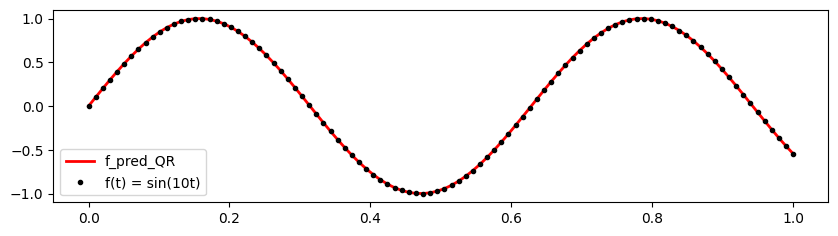
\includegraphics[width=\textwidth]{images/MGS.png}
        \caption{Fit for Modified Gram-Schmidt solutions.}
        \label{fig:image1}
    \end{minipage} \hfill
    \begin{minipage}{0.48\textwidth}
        \centering
        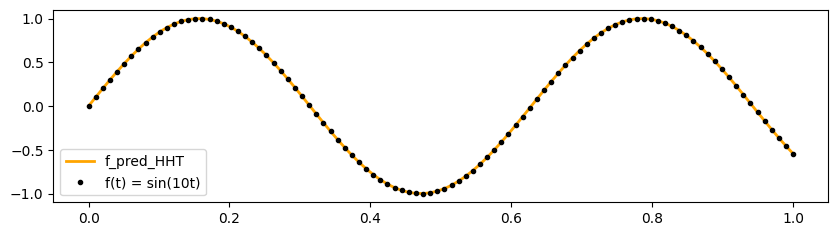
\includegraphics[width=\textwidth]{images/HHT.png}
    \caption{Fit for Householder solutions.}
        
        \label{fig:image2}
    \end{minipage}
    \vspace{0.5cm} % Adjust space between the rows

    \begin{minipage}{0.48\textwidth}
        \centering
        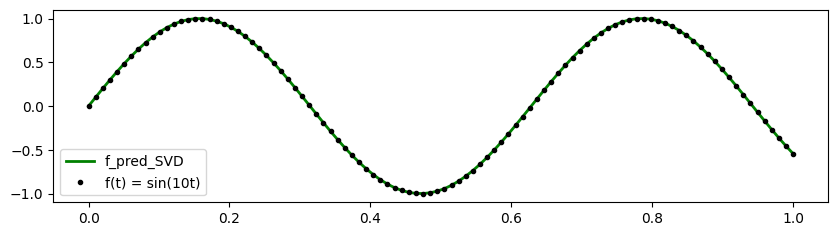
\includegraphics[width=\textwidth]{images/SVD.png}
        \caption{Fit for SVD solutions.}
        \label{fig:image3}
    \end{minipage} \hfill
    \begin{minipage}{0.48\textwidth}
        \centering
        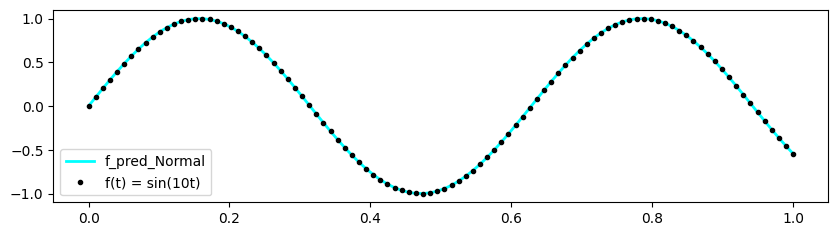
\includegraphics[width=\textwidth]{images/normal.png}
        \caption{Fit for normal equations solutions.}
        \label{fig:image4}
    \end{minipage}

    \vspace{0.5cm} % Adjust space before the last image

    \begin{minipage}{0.6\textwidth}
        \centering
        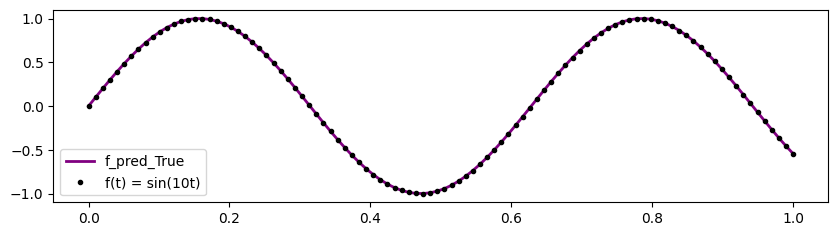
\includegraphics[width=\textwidth]{images/true.png}
        \caption{Fit for true solutions.}
        \label{fig:image5}
    \end{minipage}
    \label{fig:collection}
\end{figure}

It seems like all the functions gave an almost perfect fit. To analyze more in depth we will have to do some more fine grain analysis. 

Find the below the least squares error computed by each of the algorithm: 

\begin{table}[H]
    \centering
    \begin{tabular}{|c|c|}
        \hline
        \textbf{Method}                & \textbf{Least Squares Error} =  $\| f_{true} - f_{\text{pred}} \|_2^2$   \\ 
        \hline
        MGS                            & \( 9.402375692798181 \times 10^{-14} \) \\
        HHT                            & \( 1.1321338951663014 \times 10^{-15} \) \\
        SVD                            & \( 1.1317331635715833 \times 10^{-15} \) \\
        Normal Equations              & \( 1.8213047820333308 \times 10^{-7} \)  \\ 
        \hline
    \end{tabular}
    \caption{Comparison of Least Squares Errors for Different Methods}
    \label{tab:least_squares_error}
\end{table}

\underline{\textbf{From the table, we can make the following 3 observations:}}

\begin{enumerate}
    \item \textbf{Normal Equations} give the worst overall error.
    \item \textbf{Householder and SVD} gave comparable performances and were the best out of the 4.
    \item \textbf{MGS} gave a performance better than Normal but worse than Householder and SVD.
\end{enumerate}

We will look at the coefficients calculated for the polynomial by all the methods and compare them.

\begin{table}[H]
\centering
\begin{tabular}{|c|c|c|c|c|c|}
\hline
\textbf{i for} $a_{i}$ & \textbf{True} & \textbf{MGS} & \textbf{HHT} & \textbf{SVD} & \textbf{Normal Equations} \\
\hline
0  & -0.00000016  & -0.00000022  & -0.00000016  & -0.00000016  & 0.00009748 \\
1  & 10.00006007  & 10.00008458  & 10.00006007  & 10.00006008  & 9.97359744 \\
2  & -0.00314921  & -0.00461558  & -0.00314922  & -0.00314923  & 1.22087079 \\
3  & -166.61061960 & -166.57538541 & -166.61061941 & -166.61061922 & -189.41596248 \\
4  & -0.29594467  & -0.74497248  & -0.29594639  & -0.29594853  & 221.14580470 \\
5  & 830.45651318  & 833.92406381  & 830.45652285  & 830.45653810  & -426.59920374 \\
6  & 55.22400378  & 37.73386114  & 55.22396817  & 55.22389519  & 4421.70131727 \\
7  & -2392.04440709 & -2331.80848490 & -2392.04431955 & -2392.04407680 & -11476.49362877 \\
8  & 1801.11131016 & 1655.90668355 & 1801.11116739 & 1801.11059622 & 10999.07736950 \\
9  & -2508.83243359 & -2261.43698317 & -2508.83228716 & -2508.83133125 & 1134.97183287 \\
10 & 10530.11024551 & 10233.58080896 & 10530.11016911 & 10530.10903931 & -14650.70543866 \\
11 & -16874.05799274 & -16629.48284784 & -16874.05800110 & -16874.05708000 & 19423.64843695 \\
12 & 12787.28761695 & 12655.15373348 & 12787.28765582 & 12787.28716311 & -14452.91862230 \\
13 & -4800.45028145 & -4758.35796429 & -4800.45030375 & -4800.45014816 & 6098.23877130 \\
\textbf{14} & \textbf{727.56105819}  & \textbf{721.56799766}  & \textbf{727.56106267}  & \textbf{727.56104068}  & \textbf{-1114.38934633} \\
\hline
\end{tabular}
\caption{Comparison of coefficients computed by each method, $ith$ element represents the coefficient of $x^i$}
\label{tab:comparison_methods}
\end{table}

\begin{tcolorbox}
From the table, it is evident that Householder and SVD approximate the true values very closely. Where as MGS comes close at some of the approximation, Normal equations are giving very inaccurate values for the coefficients. 
\end{tcolorbox}



\underline{\textbf{For simplicity, we are going to compare the coefficient of $x^{14}$ for each of the methods.}}

\begin{table}[H]
\centering
\begin{minipage}{0.5\textwidth}
    \centering
    \begin{tabular}{|c|c|}
        \hline
        \textbf{Method} & \textbf{Relative Error} \\
        \hline
         MGS & 8.237193e-03 \\
         HHT & 6.151479e-09 \\
         SVD & 2.406253e-08 \\
         Normal Equations & 2.531678e+00 \\
        \hline
    \end{tabular}
    \caption{Relative Error ($x^{14}$) for Different Methods}
    \label{tab:errors}
\end{minipage}%
\hspace{0.05\textwidth} % Adjust space between tables
\begin{minipage}{0.35\textwidth}
    \centering
    \begin{tabular}{c|c|c}
        & y & x \\
        \hline
        b & 1.000000e+00 & 6.187516e+03 \\
        \hline
        A & 3.016178e+08 & 3.036732e+08 \\
    \end{tabular}
    \caption{Condition numbers of y and x with respect to perturbations in b and A.}
    \label{tab:values}
\end{minipage}
\end{table}

\textbf{At first glance, this relative error growth looks very bad. But it can be explained with the following arguments: } (remember $\epsilon_{m} \approx 2.22 \times 10 ^ {-16}$)

\begin{enumerate}
    \item \textbf{Modified Gram Schmidt}: The rounding error is roughly of the order $10^{-3}$ which means it is amplified by $10^{13}$, which is far greater than the condition number. This error can be accounted for due to \textbf{unstability}. Gram-Schmidt orthogonalization\textbf{ produces 
    matrices Q,} in general, \textbf{whose columns are not accurately orthonormal.} Since the algorithm above depends on that orthonormality, it suffers accordingly. Hence it is \textbf{UNSTABLE.}
    \\
    \item  \textbf{Householder} method (HHT): The rounding error is roughly of the order $10^{-9}$ which means it is amplified by $10^{7}$. The condition number of x w.r.t pertubation in A is roughly $3 \times 10^{8}$. \textbf{Thus the inaccuracy in $a_{14}$ can be entirely explained by ill-conditioning, not instability.} HHT is \textbf{STABLE}.
    \\
    \item \textbf{SVD} Same explanation as Householder. Error can be accounted by the condition number. SVD algo is also \textbf{STABLE}.
    \\
    \item \textbf{Normal Equations} Error growth by a factor of $10^{16}$. This can be explained by the fact that the matrix $A^TA$ has condition number is $\kappa(A)^2$ and not $\kappa(A)$.  

    $$ \frac{||\tilde{x}-x||}{||x||} = O [( \kappa(A) + \kappa(A)^2 \tan\theta / \eta) \epsilon_m]$$

    Depending on value of $\theta$ and $\eta$,  $\frac{||\tilde{x}-x||}{||x||}$ can be $\kappa(A)^2$ or $\kappa(A)$.

    Thus the behaviour of normal equations is explained by $\kappa(A)^2 \approx 10^{16}$ which amplifies the error by the given amount.

    Normal equations are typically \textbf{UNSTABLE} for \textbf{ill conditioned problems having close fits}.

    
\end{enumerate}

    \hfill \\
    \hrule

\end{question}

\end{document}


